\documentclass[11pt]{article}
\usepackage[margin=0.95in,top=0.9in,bottom=0.9in]{geometry}
\usepackage[T1]{fontenc}
\usepackage{amsmath,amssymb,amsthm}
\usepackage{booktabs}
\usepackage{graphicx}
\usepackage[compact]{titlesec}
\usepackage{hyperref}
\newtheorem{theorem}{Theorem}
\newtheorem{proposition}[theorem]{Proposition}
\theoremstyle{remark}
\newtheorem{remark}[theorem]{Remark}
\hypersetup{pdftitle={A minimum Venn diagram of order eight},pdfauthor={Chris Dzoba}}
\begin{document}
\begin{center}
{\LARGE A minimum Venn diagram of order eight}\\[10pt]
{\large Chris Dzoba}\\[4pt]
October 2026
\end{center}

\begin{abstract}
Bultena and Ruskey proved in 1998 that an $n$-Venn diagram has at least $L_n=\lceil(2^n-2)/(n-1)\rceil$ crossings
and conjectured that the bound is attained for every $n\ge 8$. We give an $8$-Venn diagram with $37=L_8$ crossings,
which settles the case $n=8$ and answers a question of Brenner, Gregor, M\"utze and Verciani; the best known before
had 39 crossings (Seamons). It has been checked by independently written programs and in Lean~4. It has a half-turn
symmetry, and no $8$-Venn diagram with 37 crossings has a larger group of orientation-preserving symmetries. Doubling gives a $9$-Venn diagram with 74
crossings, optimal among those in which some curve meets every other curve exactly twice.
\end{abstract}

\section{Introduction}

An \emph{$n$-Venn diagram} is a collection of $n$ simple closed curves in the plane that intersect in finitely many
points and create exactly $2^n$ connected regions, one for each combination of being inside or outside each curve.
In any intersection point of at least two curves at least two of them must cross, and such a point is called a
\emph{crossing} \cite{BGMV}. Several curves may pass through one crossing, and some of them may only touch there.
Bultena and Ruskey \cite{BR98} proved that an $n$-Venn diagram, $n\ge2$, has at least
$L_n=\lceil(2^n-2)/(n-1)\rceil$ crossings, called diagrams attaining the bound \emph{minimum}, and conjectured that
minimum $n$-Venn diagrams exist for all $n\ge8$ (see also \cite{RW}). They are known for $n\le7$
\cite{BR98,BGMV}. For $n=8$, $L_8=37$. Brenner, Gregor, M\"utze and Verciani \cite{BGMV} constructed an $8$-Venn
diagram with 40 crossings and asked whether 37 is possible. Seamons \cite{Sea} reduced 40 to 39 by an edge surgery
on a reconstruction of their diagram.

\begin{theorem}\label{thm:main}
There is an $8$-Venn diagram with $37$ crossings. So the least number of crossings of an $8$-Venn diagram is $37$,
and the conjecture of Bultena and Ruskey holds for $n=8$.
\end{theorem}

\section{The certificate}

We use dual graphs as in \cite[Section~1.3]{BGMV}. Let $Q_n$ be the graph on the subsets of $[n]=\{1,\dots,n\}$ in
which two sets are adjacent when they differ in one element, the \emph{direction} of the edge. The dual $Q(D)$ of an
$n$-Venn diagram $D$ has a vertex for each region, the set of curves containing it, and an edge across each arc of a
curve. It satisfies: (1) it is a spanning subgraph of $Q_n$; (2) it is a plane graph in which each face has length
$2\ell$ for some $2\le\ell\le n$ and contains exactly two edges of each of $\ell$ distinct directions; (3) for every
$j\in[n]$ the subgraphs induced by the vertices $x$ with $j\in x$ and with $j\notin x$ are connected. Conversely, the
dual of any subgraph of $Q_n$ with these properties is an $n$-Venn diagram \cite{BGMV}. The faces of $Q(D)$ are the
crossings of $D$. We work on the sphere; removing a point of a region gives a diagram in the plane.

A certificate lists the faces of a plane graph, each as the cyclic sequence of vertex labels around it, with
$x\subseteq[n]$ stored as $\sum_{i\in x}2^{i-1}$; so curve $i$ is bit $i-1$ in the files, the Lean code and the
legend of Figure~\ref{fig:diagram}. The certificate \texttt{venn8\_37\_halfturn\_a.json} (SHA-256
\texttt{7c1fed92\dots c41dd12}) has 256 vertices, 291 edges and 37 faces, 32 of length 16 and five of length 14. So
32 crossings lie on all eight curves and five on seven. Curves 1, 3, 5, 7 and 8 pass through all 37 crossings, curve
4 through 36, curves 2 and 6 through 35. At every crossing some pair of curves crosses.

\begin{figure}[t]
\centering
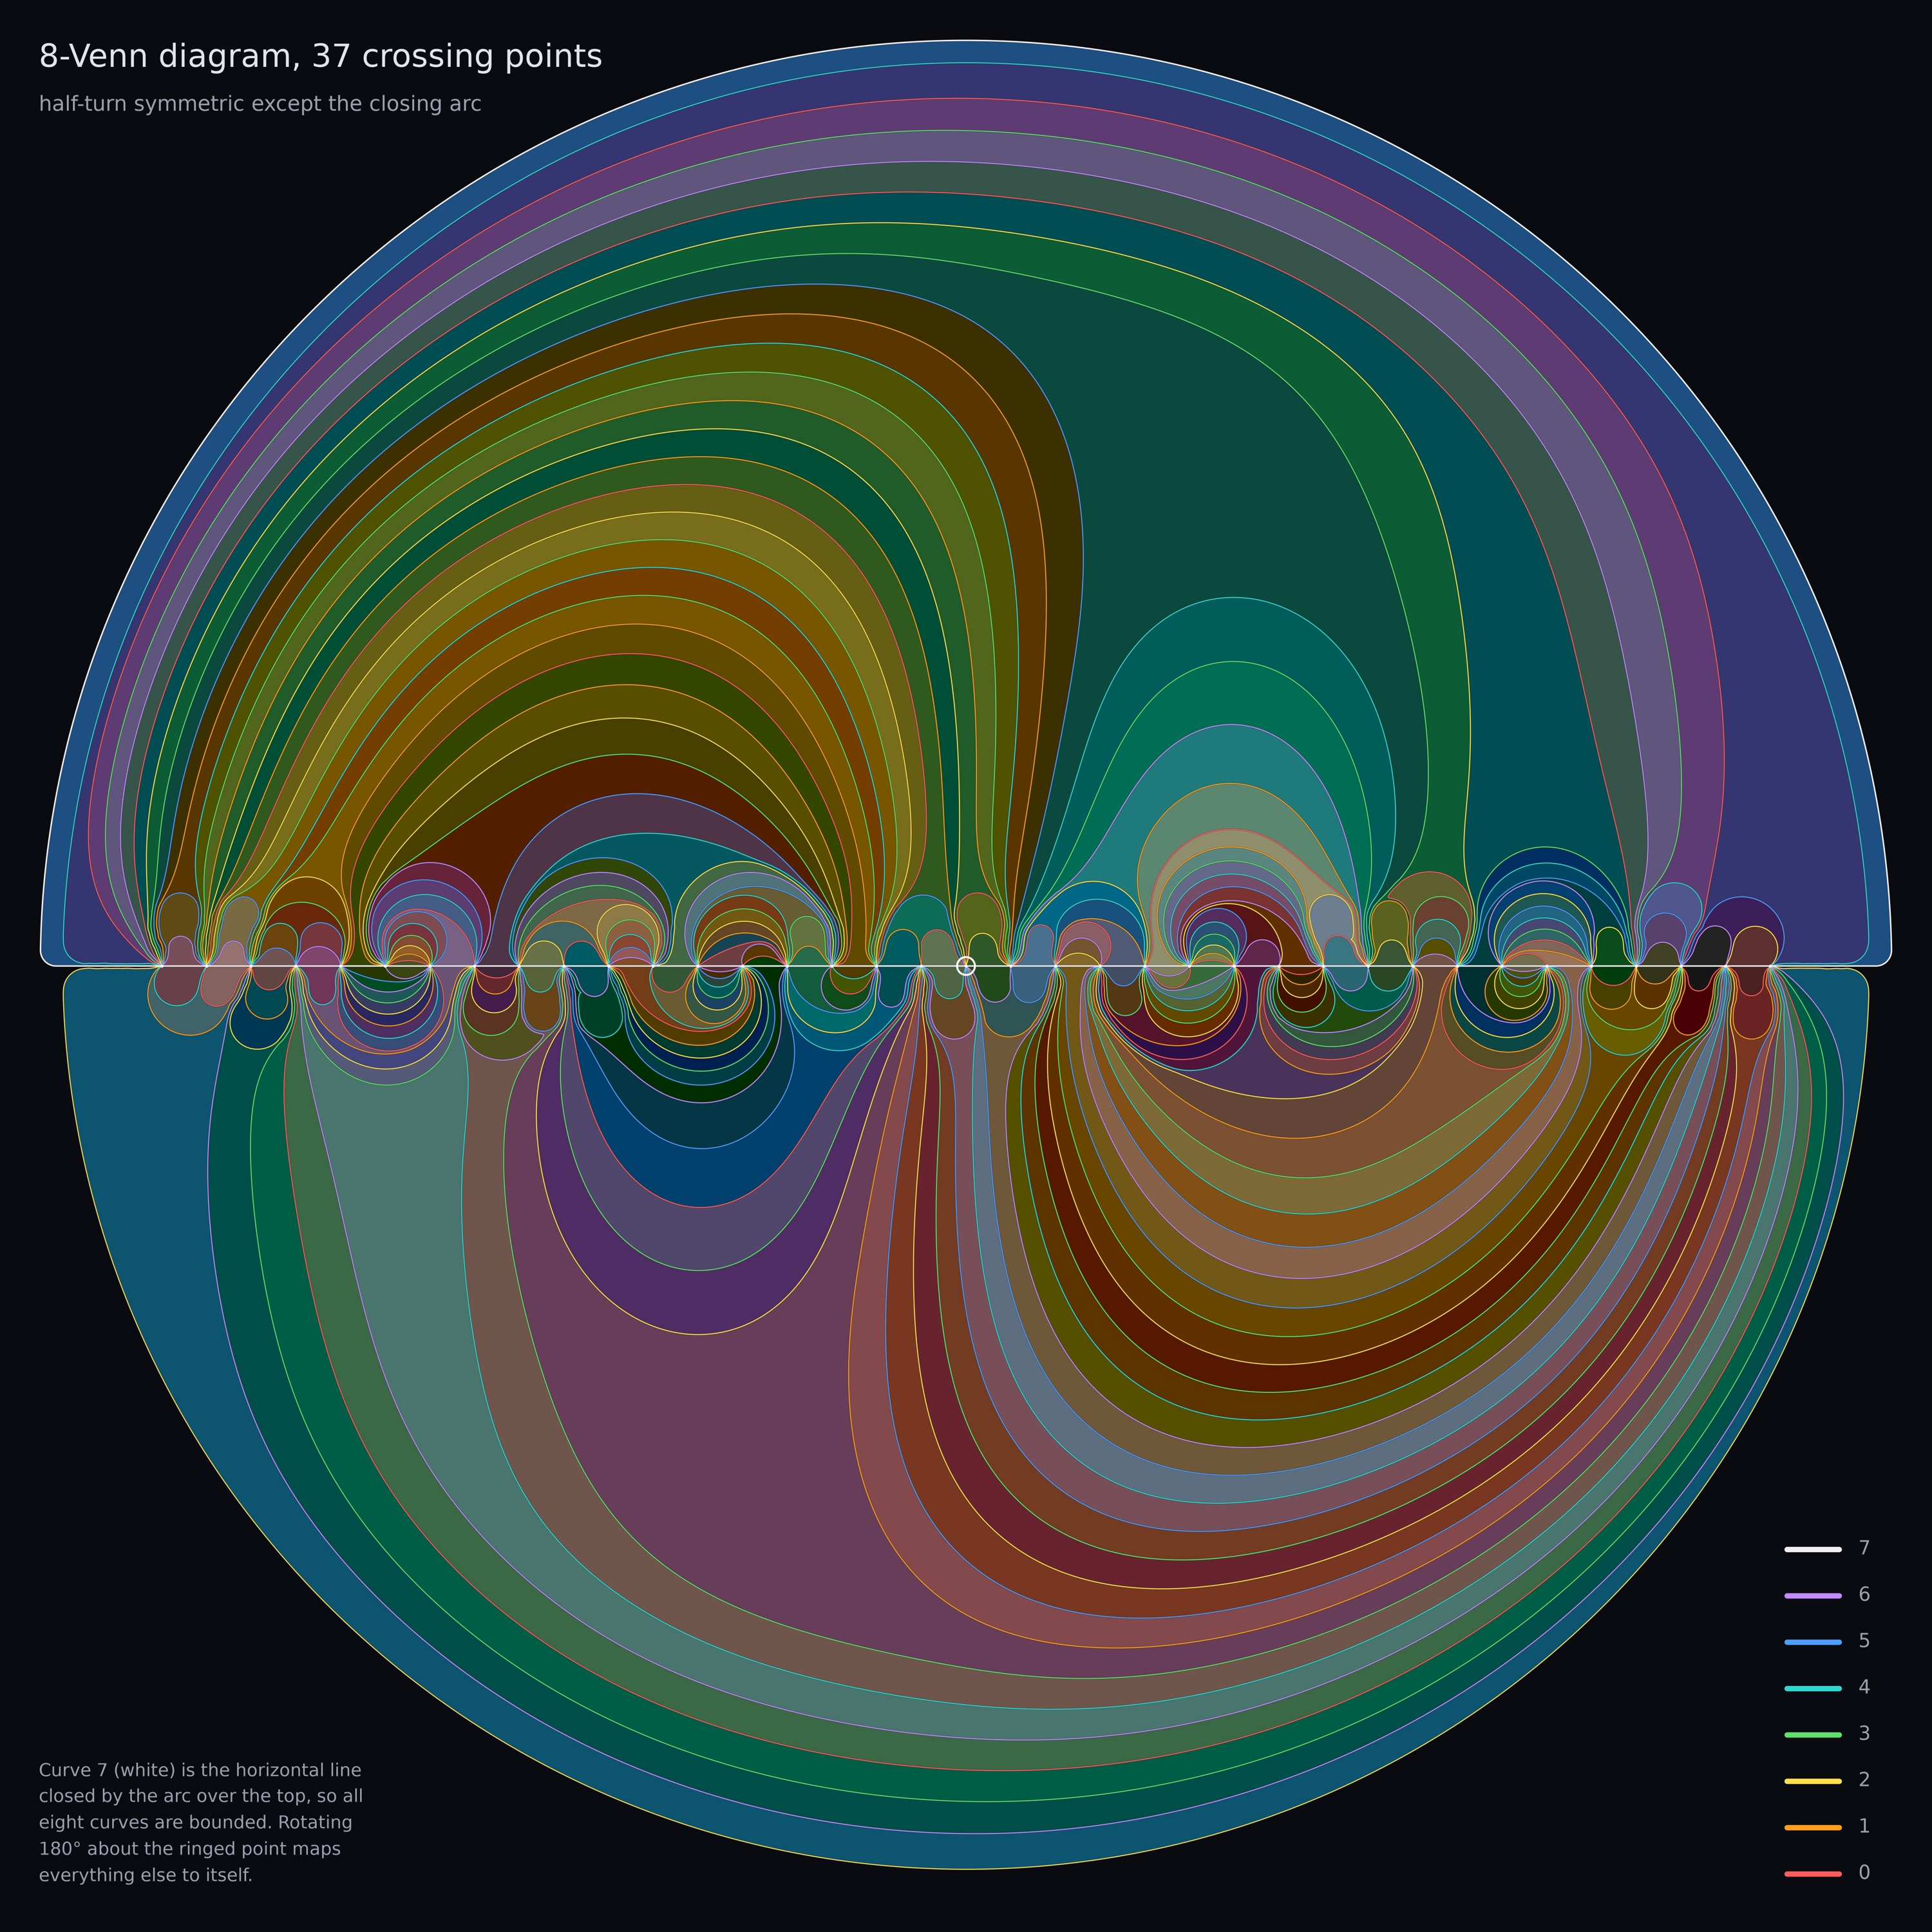
\includegraphics[width=0.44\textwidth]{venn8_37.jpg}
\caption{The diagram of \texttt{venn8\_37\_halfturn\_a.json}, drawn and checked against the certificate by
\texttt{render37.py}. Curve $j$ of the legend is curve $j+1$ in the text; curve 8 (white) is the line closed by the arc
over the top. Rotation by $180^\circ$ about the ringed crossing preserves the drawing except along that arc.}
\label{fig:diagram}
\end{figure}

\section{The lower bound and the checks}

We recall why 37 is least \cite{BR98}. The dual of an $n$-Venn diagram is a connected plane graph with $V=2^n$
vertices, $E$ edges and $F$ faces, so $V-E+F=2$. Face lengths are at most $2n$ and sum to $2E$, so $E\le nF$ and
$2^n-2=E-F\le(n-1)F$, hence $F\ge L_n$. For $n=8$, $F\ge\lceil254/7\rceil=37$, and $F=37$ forces $E=291$ and
$\sum_f(8-\ell_f)=5$, where $2\ell_f$ is the length of face $f$.

The repository accompanying this note contains the certificates, three checkers and their logs, the Lean project
and the drawing program. Theorem~\ref{thm:main} reduces to checking that 37 faces satisfy (1)--(3) and form a plane
graph. Three separately written checkers do this in a fraction of a second: \texttt{check\_a.py} checks (1)--(3), the induced
rotation system and Euler's formula; \texttt{check\_b.py} builds the primal diagram and checks that the arcs of each
curve form one closed curve; \texttt{ref37\_v2.py}, written from scratch by a separate referee, also checks that
some pair of curves crosses at each crossing. All three accept both 37-crossing certificates, Seamons's 39 and his
reconstruction of the 40 of \cite{BGMV}, and reject each of these with a face removed (\texttt{python3
checkers/run\_all.py}). Two checkers written by Codex also accept both 37-crossing certificates.

For the face list \texttt{cert} of \texttt{venn8\_37\_halfturn\_a.json}, a Lean~4 proof (with Mathlib) in
\texttt{lean/} establishes
\begin{center}\footnotesize
\texttt{(IsVennDual8 cert}\ $\wedge$\ \texttt{CrossingAtEachPoint cert)}\ $\wedge$\ \texttt{cert.length = 37}\
$\wedge$\\ $\forall$\,\texttt{fs, IsVennDual8 fs}\ $\to$\ \texttt{37}\ $\le$\ \texttt{fs.length}.
\end{center}
\texttt{IsVennDual8} states (1)--(3) for an oriented face list and that the list is a combinatorial map of the
sphere (each edge traversed once in each direction, vertex links single cycles, connected, $V-E+F=2$);
\texttt{CrossingAtEachPoint} says that two directions interleave on every face. The facts about \texttt{cert} are
proved by kernel evaluation (\texttt{decide +kernel}), the bound by a general argument, using only the axioms
\texttt{propext}, \texttt{Classical.choice} and \texttt{Quot.sound}. The characterization of \cite{BGMV} and the
passage from a combinatorial map to a drawing are cited, not formalized.

\section{Symmetry and a second diagram}\label{sec:sym}

A symmetry of a diagram on the sphere is a homeomorphism mapping the set of curves onto itself. It acts on labels by
$x\mapsto\pi(x)\mathbin{\triangle}c$ for a permutation $\pi$ of $[n]$ and a set $c\subseteq[n]$. With
$\sigma=(1\,7)(2\,6)(3\,5)$ and $c=[8]\setminus\{4\}$ (the integer 247), $g(x)=\sigma(x)\mathbin{\triangle}c$ maps
every face of \texttt{venn8\_37\_halfturn\_a.json} to a face with the same orientation: a half-turn. It fixes no
region, one arc (dual to the edge between $\{5,6,7\}$ and $\{5,6,7,8\}$, on curve 8) and one crossing, on all curves but curve 4. A
search over all maps $x\mapsto\pi(x)\mathbin{\triangle}c$ finds no other automorphism of the face list.

\begin{proposition}\label{prop:rot}
Let $G$ be a finite group of orientation-preserving symmetries of an $8$-Venn diagram with $37$ crossings. Then
$|G|\le2$, and a symmetry of order $2$ fixes exactly one crossing, one arc and no region.
\end{proposition}

\begin{proof}
The 37 crossings, 291 arcs and 256 regions are the cells of a decomposition of the sphere. Let $g\in G$ have order
$k\ge2$. By Ker\'ekj\'art\'o's theorem \cite{CK} $g$ is conjugate to a rotation, whose two poles are the only fixed
points of each nontrivial power of $g$. A cell mapped to itself by such a power contains a fixed point of it (for an
arc since a periodic map of an interval has one, for a region by \cite{CK} on its one-point compactification), so
the cells without a pole lie in orbits of size $k$. If $v,e,f$ count the regions, arcs and crossings containing a
pole, then $v+e+f\le2$ and $256\equiv v$, $291\equiv e$, $37\equiv f\pmod k$. If $k\ge3$ then $e=0$: an arc containing
a pole would be mapped to itself, and as a periodic map of an interval has order at most 2, the nontrivial $g^2$
would fix the whole arc. So $k\mid291=3\cdot97$. For
$k\in\{97,291\}$, $256\bmod k\in\{62,256\}$ exceeds $v\le2$. For $k=3$, $v=1$; but the fixed labels, solutions of
$\pi(x)\mathbin{\triangle}c=x$, form a coset of a subspace of $\mathbb{F}_2^8$ of dimension the number of cycles of
$\pi$, so there are $0$ or at least $2$. Hence $k=2$, and parity gives $(v,e,f)=(0,1,1)$. So $G$ is an elementary
abelian $2$-group. Its orbits on the 37 crossings have size a power of 2, so it fixes a crossing, and it acts
faithfully by rotations on the cyclic sequence of regions around it, since no nontrivial element fixes a region.
So $G$ is cyclic and $|G|\le2$.
\end{proof}

\begin{remark}
Orientation-reversing symmetries are also impossible, so the full group is trivial or of order 2. In outline: a
reversing involution fixes a crossing, so it is a reflection in a circle $M$ \cite{CK}. Its permutation $\pi$ fixes
an even number $s$ of curves, and each of these meets $M$ twice if its sides are kept. A curve with its sides
exchanged would equal $M$ and meet another fixed curve only twice, but any two curves share at least 32 crossings.
Otherwise the Lefschetz number gives $f+a-v=0$ for the invariant crossings, arcs and regions, where $f$ is odd,
$a\le2s$, $v\in\{0,2^{(8+s)/2}\}$ and $f\le7$ if $s>0$; no case fits. An element of order 4 would square to the
half-turn and fix its invariant arc pointwise. This is not formalized.
\end{remark}

The certificate \texttt{venn8\_37\_halfturn\_b.json} is a second diagram with 37 crossings, with the same face
lengths and symmetry $g$. It is not isomorphic to the first, even allowing relabelling of curves, exchange of inside
and outside, and reflection: the numbers of crossings on the curves are $34,36,36,37,37,37,37,37$ against
$35,35,36,37,37,37,37,37$, and the dual graphs have $196$, $50$, $10$ vertices of degree $2$, $3$, $4$ against
$192$, $58$, $6$.

\section{Nine and more curves}\label{sec:nine}

A face of the dual is \emph{colorful} if it has length $2n$ and contains complementary vertices $x$ and
$[n]\setminus x$. By \cite[Lemma~11]{BGMV}, a diagram whose dual has a colorful face gives an $(n+1)$-Venn diagram
with twice as many crossings and again a colorful face: two copies of the dual, the second with $n+1$ added to every
label, are joined by the edges $\{x,x\cup\{n+1\}\}$ and $\{\bar x,\bar x\cup\{n+1\}\}$ for complementary $x,\bar x$ on
that face. The face of
\texttt{venn8\_37\_halfturn\_a.json} containing $\{6,7,8\}$ and $\{1,\dots,5\}$ is colorful, which gives $n$-Venn
diagrams with $37\cdot2^{n-8}$ crossings (Table~\ref{tab:double}; for $n=16$ the 5118 of \cite{BGMV} is smaller).
The 9-Venn diagram \texttt{venn9\_74.json} also passes the two checkers of Codex. The files for $10\le n\le15$ were
checked only by the three programs in \texttt{checkers/}; \texttt{checkers/invariants.py} confirms that each is the
doubling of the previous one.

\begin{table}[h]
\centering\small
\begin{tabular}{lrrrrrrrr}
\toprule
$n$ & 8 & 9 & 10 & 11 & 12 & 13 & 14 & 15\\
\midrule
lower bound $L_n$ \cite{BR98} & 37 & 64 & 114 & 205 & 373 & 683 & 1261 & 2341\\
\cite[Theorem~2]{BGMV} & 40 & 80 & 160 & 320 & 640 & 1280 & 2560 & 5120\\
this note & 37 & 74 & 148 & 296 & 592 & 1184 & 2368 & 4736\\
\bottomrule
\end{tabular}
\caption{Numbers of crossings; for $n\ge9$ the last row is by doubling (Seamons's 39 gives 78).}
\label{tab:double}
\end{table}

In \texttt{venn9\_74.json} curve 9 meets every other curve in exactly two points. In this class 74 is optimal.

\begin{proposition}\label{prop:class}
Let $n\ge3$, $m=n-1$, and let an $n$-Venn diagram with $F$ crossings have a curve $c$ that meets every other curve in
exactly two points. If $k$ crossings lie on $c$, then $F\ge2(L_m-1)+k\ge2L_m$; for $n=9$, $F\ge74$.
\end{proposition}

\begin{proof}
Another curve $j$ meets $c$ in two points $p,q$, and has points on both sides of $c$, so one of its arcs between $p$
and $q$ lies inside $c$ and the other outside. Let $\Delta$ be the closed disc bounded by $c$ on one side, and
collapse $c$ to a point $P$. The other $m$ curves become simple closed curves through $P$, whose union is a connected
plane graph with vertices $P$ and the $I$ crossings inside $\Delta$, all of degree at most $2m$, and with the $2^m$
regions inside $\Delta$ as faces. Euler's formula gives $2^m-2=E-(I+1)\le(m-1)(I+1)$, so $I+1\ge L_m$. The same holds
on the other side, and $k\ge2$ crossings lie on $c$, so $F\ge2(L_m-1)+k$.
\end{proof}

This bounds one class only; in general only $L_9=64$ is known. Our search also found 74-crossing $9$-Venn diagrams
outside the class (\texttt{venn9\_74\_mixed\_r2.json}, \texttt{venn9\_74\_k3\_nearmiss.json}), and none with fewer
than 74 crossings.

\paragraph{How the diagrams were found.} A Metropolis walk over plane spanning subgraphs of $Q_8$, given as rotation
systems, allowed unbalanced faces and disconnected curve halves at a cost and applied each move together with its
image under $g$. From half-turn invariant arrangements of the nested cycles of \cite{BGMV} it produced many diagrams
with 38 and 39 crossings, and walks from two 39s with a higher cost per edge reached the two 37s. The search programs
are not included.

\section*{Use of AI tools}
This work was carried out with AI systems under the author's direction. Claude (Anthropic) wrote and ran the searches,
the checkers \texttt{check\_a.py} and \texttt{check\_b.py}, the doubling and the drawing, wrote the Lean
formalization, and drafted the text; a separate Claude instance wrote \texttt{ref37\_v2.py}. The proofs of
Sections~\ref{sec:sym} and~\ref{sec:nine} were worked out by Claude and Codex (OpenAI). Codex contributed the
exclusion of reflections and reviewed Proposition~\ref{prop:class}, wrote two further checkers and a reconstruction
of the first diagram, checked both 37-crossing diagrams and the 74-crossing diagram, and rebuilt and reviewed the Lean
proof. The author is responsible for the content.

\small
\begin{thebibliography}{9}\setlength{\itemsep}{0pt}
\bibitem{BGMV} S.~Brenner, P.~Gregor, T.~M\"utze and F.~Verciani, On minimum Venn diagrams, \emph{SoCG 2026},
LIPIcs 367 (2026), 21:1--21:18; arXiv:2511.09230.
\bibitem{BR98} B.~Bultena and F.~Ruskey, Venn diagrams with few vertices, \emph{Electron. J. Combin.} 5 (1998),
\#R44.
\bibitem{CK} A.~Constantin and B.~Kolev, The theorem of Ker\'ekj\'art\'o on periodic homeomorphisms of the disc and
the sphere, \emph{Enseign. Math.} (2) 40 (1994), 193--204.
\bibitem{RW} F.~Ruskey and M.~Weston, A survey of Venn diagrams, \emph{Electron. J. Combin.}, Dynamic Survey DS5.
\bibitem{Sea} J.~Seamons, A 39-crossing Venn diagram of order eight, Zenodo (2026), doi:10.5281/zenodo.22004839.
\end{thebibliography}
\end{document}
